\documentclass[twoside]{book}

% Packages required by doxygen
\usepackage{fixltx2e}
\usepackage{calc}
\usepackage{doxygen}
\usepackage[export]{adjustbox} % also loads graphicx
\usepackage{graphicx}
\usepackage[utf8]{inputenc}
\usepackage{makeidx}
\usepackage{multicol}
\usepackage{multirow}
\PassOptionsToPackage{warn}{textcomp}
\usepackage{textcomp}
\usepackage[nointegrals]{wasysym}
\usepackage[table]{xcolor}

% NLS support packages
\usepackage[spanish]{babel}
% Font selection
\usepackage[T1]{fontenc}
\usepackage[scaled=.90]{helvet}
\usepackage{courier}
\usepackage{amssymb}
\usepackage{sectsty}
\renewcommand{\familydefault}{\sfdefault}
\allsectionsfont{%
  \fontseries{bc}\selectfont%
  \color{darkgray}%
}
\renewcommand{\DoxyLabelFont}{%
  \fontseries{bc}\selectfont%
  \color{darkgray}%
}
\newcommand{\+}{\discretionary{\mbox{\scriptsize$\hookleftarrow$}}{}{}}

% Page & text layout
\usepackage{geometry}
\geometry{%
  a4paper,%
  top=2.5cm,%
  bottom=2.5cm,%
  left=2.5cm,%
  right=2.5cm%
}
\tolerance=750
\hfuzz=15pt
\hbadness=750
\setlength{\emergencystretch}{15pt}
\setlength{\parindent}{0cm}
\setlength{\parskip}{3ex plus 2ex minus 2ex}
\makeatletter
\renewcommand{\paragraph}{%
  \@startsection{paragraph}{4}{0ex}{-1.0ex}{1.0ex}{%
    \normalfont\normalsize\bfseries\SS@parafont%
  }%
}
\renewcommand{\subparagraph}{%
  \@startsection{subparagraph}{5}{0ex}{-1.0ex}{1.0ex}{%
    \normalfont\normalsize\bfseries\SS@subparafont%
  }%
}
\makeatother

% Headers & footers
\usepackage{fancyhdr}
\pagestyle{fancyplain}
\fancyhead[LE]{\fancyplain{}{\bfseries\thepage}}
\fancyhead[CE]{\fancyplain{}{}}
\fancyhead[RE]{\fancyplain{}{\bfseries\leftmark}}
\fancyhead[LO]{\fancyplain{}{\bfseries\rightmark}}
\fancyhead[CO]{\fancyplain{}{}}
\fancyhead[RO]{\fancyplain{}{\bfseries\thepage}}
\fancyfoot[LE]{\fancyplain{}{}}
\fancyfoot[CE]{\fancyplain{}{}}
\fancyfoot[RE]{\fancyplain{}{\bfseries\scriptsize Generado por Doxygen }}
\fancyfoot[LO]{\fancyplain{}{\bfseries\scriptsize Generado por Doxygen }}
\fancyfoot[CO]{\fancyplain{}{}}
\fancyfoot[RO]{\fancyplain{}{}}
\renewcommand{\footrulewidth}{0.4pt}
\renewcommand{\chaptermark}[1]{%
  \markboth{#1}{}%
}
\renewcommand{\sectionmark}[1]{%
  \markright{\thesection\ #1}%
}

% Indices & bibliography
\usepackage{natbib}
\usepackage[titles]{tocloft}
\setcounter{tocdepth}{3}
\setcounter{secnumdepth}{5}
\makeindex

% Hyperlinks (required, but should be loaded last)
\usepackage{ifpdf}
\ifpdf
  \usepackage[pdftex,pagebackref=true]{hyperref}
\else
  \usepackage[ps2pdf,pagebackref=true]{hyperref}
\fi
\hypersetup{%
  colorlinks=true,%
  linkcolor=blue,%
  citecolor=blue,%
  unicode%
}

% Custom commands
\newcommand{\clearemptydoublepage}{%
  \newpage{\pagestyle{empty}\cleardoublepage}%
}

\usepackage{caption}
\captionsetup{labelsep=space,justification=centering,font={bf},singlelinecheck=off,skip=4pt,position=top}

%===== C O N T E N T S =====

\begin{document}

% Titlepage & ToC
\hypersetup{pageanchor=false,
             bookmarksnumbered=true,
             pdfencoding=unicode
            }
\pagenumbering{roman}
\begin{titlepage}
\vspace*{7cm}
\begin{center}%
{\Large Práctica 1 -\/ S\+O\+P\+ER }\\
\vspace*{1cm}
{\large Generado por Doxygen 1.8.11}\\
\end{center}
\end{titlepage}
\clearemptydoublepage
\tableofcontents
\clearemptydoublepage
\pagenumbering{arabic}
\hypersetup{pageanchor=true}

%--- Begin generated contents ---
\chapter{Índice de estructura de datos}
\section{Estructura de datos}
Lista de estructuras con una breve descripción\+:\begin{DoxyCompactList}
\item\contentsline{section}{\hyperlink{structmatrix}{matrix} }{\pageref{structmatrix}}{}
\end{DoxyCompactList}

\chapter{Indice de archivos}
\section{Lista de archivos}
Lista de todos los archivos documentados y con descripciones breves\+:\begin{DoxyCompactList}
\item\contentsline{section}{\hyperlink{ejercicio10_8c}{ejercicio10.\+c} \\*Fuente del ejercicio 10 }{\pageref{ejercicio10_8c}}{}
\item\contentsline{section}{\hyperlink{ejercicio10b_8c}{ejercicio10b.\+c} \\*Fuente del ejercicio 10, versión2 }{\pageref{ejercicio10b_8c}}{}
\item\contentsline{section}{\hyperlink{ejercicio3a_8c}{ejercicio3a.\+c} \\*Fuente del ejercicio 3a }{\pageref{ejercicio3a_8c}}{}
\item\contentsline{section}{\hyperlink{ejercicio3b_8c}{ejercicio3b.\+c} \\*Fuente del ejercicio 3b }{\pageref{ejercicio3b_8c}}{}
\item\contentsline{section}{\hyperlink{ejercicio4_8c}{ejercicio4.\+c} \\*Fuente del ejercicio 4 Este programa pide al usuario dos matrices y dos factores para multiplicarlas. Multiplica cada una por un factor en dos hilos distintos que además mantienen una comunicación para saber por donde va el otro }{\pageref{ejercicio4_8c}}{}
\item\contentsline{section}{\hyperlink{ejercicio8_8c}{ejercicio8.\+c} \\*Fuente del ejercicio 8 Este programa pide al usuario un número de procesos y un número de vueltas, estos procesos se pasarán una señal tantas vueltas como pida el usuario. Cada vez que uno la recibe, imprime la hora. Finalmente se acaban uno a uno }{\pageref{ejercicio8_8c}}{}
\end{DoxyCompactList}

\chapter{Documentación de las estructuras de datos}
\hypertarget{struct__info}{}\section{Referencia de la Estructura \+\_\+info}
\label{struct__info}\index{\+\_\+info@{\+\_\+info}}
\subsection*{Campos de datos}
\begin{DoxyCompactItemize}
\item 
char {\bfseries nombre} \mbox{[}80\mbox{]}\hypertarget{struct__info_acdcd46bce5e23ab67113d7de0033169d}{}\label{struct__info_acdcd46bce5e23ab67113d7de0033169d}

\item 
int {\bfseries id}\hypertarget{struct__info_aad251c67a1f0bce28b975a9d36fc0f4a}{}\label{struct__info_aad251c67a1f0bce28b975a9d36fc0f4a}

\end{DoxyCompactItemize}


La documentación para esta estructura fue generada a partir del siguiente fichero\+:\begin{DoxyCompactItemize}
\item 
\hyperlink{ejercicio2_8c}{ejercicio2.\+c}\end{DoxyCompactItemize}

\chapter{Documentación de archivos}
\hypertarget{ejercicio2_8c}{}\section{Referencia del Archivo ejercicio2.\+c}
\label{ejercicio2_8c}\index{ejercicio2.\+c@{ejercicio2.\+c}}


Fuente del ejercicio 2.  


{\ttfamily \#include $<$stdio.\+h$>$}\\*
{\ttfamily \#include $<$stdlib.\+h$>$}\\*
{\ttfamily \#include $<$sys/ipc.\+h$>$}\\*
{\ttfamily \#include $<$sys/shm.\+h$>$}\\*
{\ttfamily \#include $<$sys/types.\+h$>$}\\*
{\ttfamily \#include $<$signal.\+h$>$}\\*
{\ttfamily \#include $<$sys/wait.\+h$>$}\\*
{\ttfamily \#include $<$errno.\+h$>$}\\*
{\ttfamily \#include $<$time.\+h$>$}\\*
{\ttfamily \#include $<$string.\+h$>$}\\*
Dependencia gráfica adjunta para ejercicio2.\+c\+:
\nopagebreak
\begin{figure}[H]
\begin{center}
\leavevmode
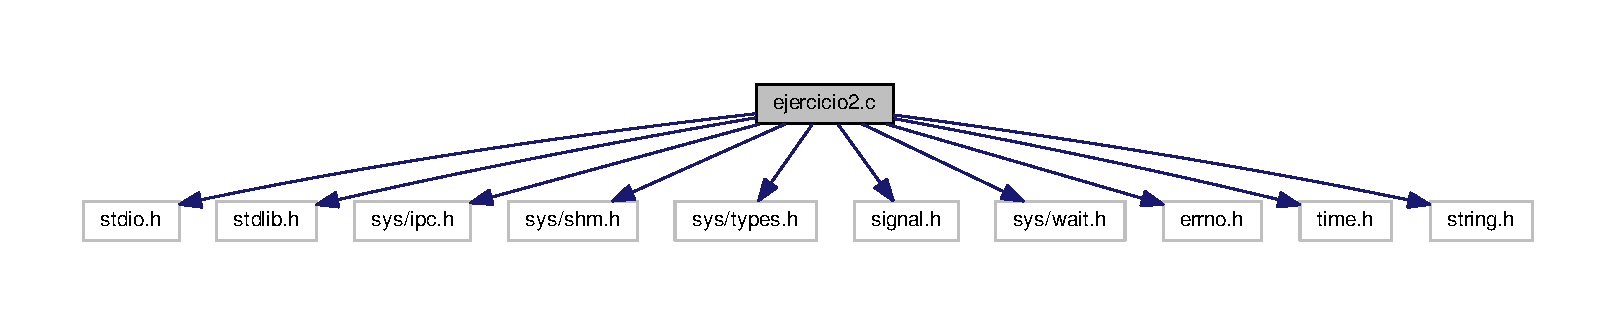
\includegraphics[width=350pt]{ejercicio2_8c__incl}
\end{center}
\end{figure}
\subsection*{Estructuras de datos}
\begin{DoxyCompactItemize}
\item 
struct \hyperlink{struct__info}{\+\_\+info}
\end{DoxyCompactItemize}
\subsection*{\textquotesingle{}defines\textquotesingle{}}
\begin{DoxyCompactItemize}
\item 
\#define {\bfseries M\+A\+X\+B\+UF}~500\hypertarget{ejercicio2_8c_ad7871643c05865c80f5d8050aead2b57}{}\label{ejercicio2_8c_ad7871643c05865c80f5d8050aead2b57}

\item 
\#define {\bfseries P\+R\+O\+J\+ID}~1300\hypertarget{ejercicio2_8c_a489440928d1b279bb8bdc0bb2ccd414f}{}\label{ejercicio2_8c_a489440928d1b279bb8bdc0bb2ccd414f}

\item 
\#define {\bfseries M\+A\+X\+U\+S\+EC}~10000\hypertarget{ejercicio2_8c_a8029636f0ea4810d2d33cca7199f00e6}{}\label{ejercicio2_8c_a8029636f0ea4810d2d33cca7199f00e6}

\end{DoxyCompactItemize}
\subsection*{\textquotesingle{}typedefs\textquotesingle{}}
\begin{DoxyCompactItemize}
\item 
typedef struct \hyperlink{struct__info}{\+\_\+info} {\bfseries Info}\hypertarget{ejercicio2_8c_ad9bb305d1fe54a0baff3b4e75119e4ee}{}\label{ejercicio2_8c_ad9bb305d1fe54a0baff3b4e75119e4ee}

\end{DoxyCompactItemize}
\subsection*{Funciones}
\begin{DoxyCompactItemize}
\item 
void {\bfseries handler\+\_\+sigusr1} ()\hypertarget{ejercicio2_8c_ae6e016b7ab83e7050bb0005c17fd13bc}{}\label{ejercicio2_8c_ae6e016b7ab83e7050bb0005c17fd13bc}

\item 
int {\bfseries main} (int argc, char $\ast$argv\mbox{[}$\,$\mbox{]})\hypertarget{ejercicio2_8c_a0ddf1224851353fc92bfbff6f499fa97}{}\label{ejercicio2_8c_a0ddf1224851353fc92bfbff6f499fa97}

\end{DoxyCompactItemize}


\subsection{Descripción detallada}
Fuente del ejercicio 2. 

Este programa reserva una zona dememoria compartida, y crea una serie de hijos, tantos como se le indique por parámetros. Cada uno de los hijos altera la memoria compartida, envia una señal al padre y termina. El padre por su parte cada vez que recibe esa señal, lee de la memoria compartida, imprime el contenido por pantalla y termina. Cabe destacar que este ejercicio tiene un fallo en su planteamiento, al no controlar la concurrencia de ninguna manera.

Para ejecutarse, se debe utilizar el comando\+:

./ejercicio2 N

Donde N será el número de hijos a crear.

\begin{DoxyAuthor}{Autor}
Juan Riera Gomez (\href{mailto:juan.riera@estudiante.uam.es}{\tt juan.\+riera@estudiante.\+uam.\+es}) y Carlos Ignacio Isasa Martín (\href{mailto:carlos.isasa@estudiante.uam.es}{\tt carlos.\+isasa@estudiante.\+uam.\+es}) 
\end{DoxyAuthor}
\begin{DoxyVersion}{Versión}
1.\+0 
\end{DoxyVersion}
\begin{DoxyDate}{Fecha}
06-\/abril-\/2017 
\end{DoxyDate}

\hypertarget{ejercicio5_8c}{}\section{Referencia del Archivo ejercicio5.\+c}
\label{ejercicio5_8c}\index{ejercicio5.\+c@{ejercicio5.\+c}}


Fuente del ejercicio 5.  


{\ttfamily \#include $<$stdio.\+h$>$}\\*
{\ttfamily \#include $<$stdlib.\+h$>$}\\*
{\ttfamily \#include \char`\"{}semaforos.\+h\char`\"{}}\\*
Dependencia gráfica adjunta para ejercicio5.\+c\+:
\nopagebreak
\begin{figure}[H]
\begin{center}
\leavevmode
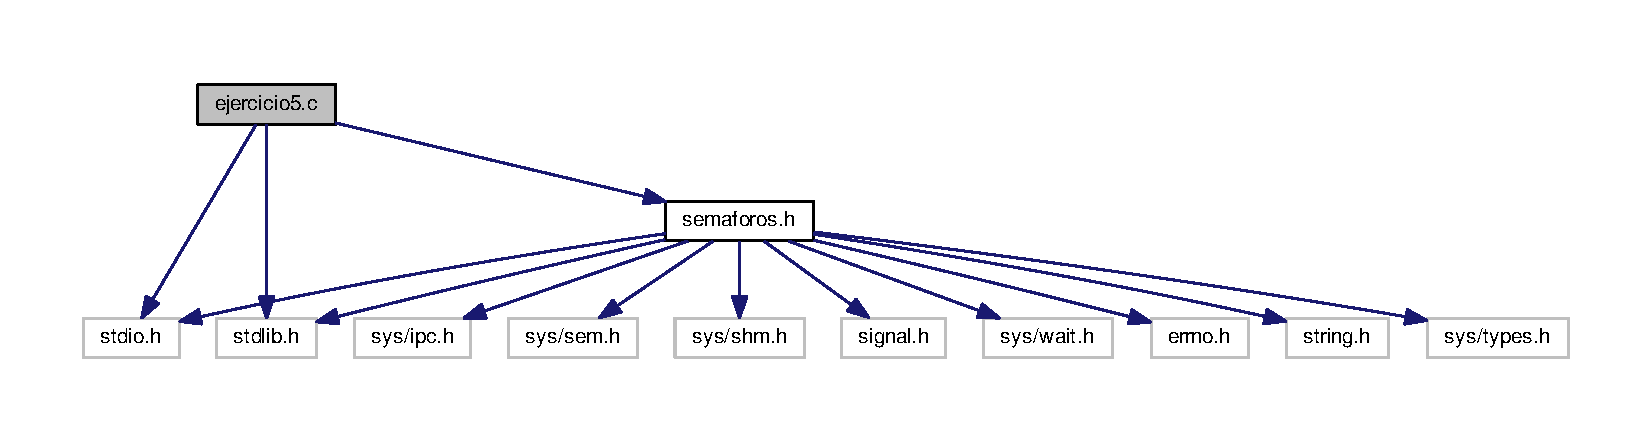
\includegraphics[width=350pt]{ejercicio5_8c__incl}
\end{center}
\end{figure}
\subsection*{\textquotesingle{}defines\textquotesingle{}}
\begin{DoxyCompactItemize}
\item 
\#define {\bfseries P\+R\+O\+J\+ID}~1301\hypertarget{ejercicio5_8c_a489440928d1b279bb8bdc0bb2ccd414f}{}\label{ejercicio5_8c_a489440928d1b279bb8bdc0bb2ccd414f}

\item 
\#define {\bfseries U\+N\+I\+Q\+U\+E\+P\+A\+TH}~\char`\"{}fichero.\+txt\char`\"{}\hypertarget{ejercicio5_8c_a558cc404f5a64ed800e9e780eae7e978}{}\label{ejercicio5_8c_a558cc404f5a64ed800e9e780eae7e978}

\item 
\#define {\bfseries S\+E\+M\+N\+UM}~5\hypertarget{ejercicio5_8c_a61727cec33cebd106b7ef8fe9e371548}{}\label{ejercicio5_8c_a61727cec33cebd106b7ef8fe9e371548}

\end{DoxyCompactItemize}
\subsection*{Funciones}
\begin{DoxyCompactItemize}
\item 
int {\bfseries main} ()\hypertarget{ejercicio5_8c_ae66f6b31b5ad750f1fe042a706a4e3d4}{}\label{ejercicio5_8c_ae66f6b31b5ad750f1fe042a706a4e3d4}

\end{DoxyCompactItemize}


\subsection{Descripción detallada}
Fuente del ejercicio 5. 

Este programa se encarga de testear la libreria de \hyperlink{semaforos_8c}{semaforos.\+c}. Su estructura general consiste en ejecutar cada una de las funciones de la libreria, comprobando que ésta no devuelve error y después pedirle al sistema que nos dé los valores actuales del semáforo, para comprobar que está todo en orden. Además se notifica al usuario por línea de comandos el estado actual del test, y si ha habido algún error.

\begin{DoxyAuthor}{Autor}
Juan Riera Gomez (\href{mailto:juan.riera@estudiante.uam.es}{\tt juan.\+riera@estudiante.\+uam.\+es}) y Carlos Ignacio Isasa Martín (\href{mailto:carlos.isasa@estudiante.uam.es}{\tt carlos.\+isasa@estudiante.\+uam.\+es}) 
\end{DoxyAuthor}
\begin{DoxyVersion}{Versión}
1.\+0 
\end{DoxyVersion}
\begin{DoxyDate}{Fecha}
06-\/abril-\/2017 
\end{DoxyDate}

\hypertarget{ejercicio6_8c}{}\section{Referencia del Archivo ejercicio6.\+c}
\label{ejercicio6_8c}\index{ejercicio6.\+c@{ejercicio6.\+c}}


Fuente del ejercicio 6.  


{\ttfamily \#include $<$stdio.\+h$>$}\\*
{\ttfamily \#include $<$stdlib.\+h$>$}\\*
{\ttfamily \#include $<$sys/ipc.\+h$>$}\\*
{\ttfamily \#include $<$sys/shm.\+h$>$}\\*
{\ttfamily \#include $<$sys/types.\+h$>$}\\*
{\ttfamily \#include $<$unistd.\+h$>$}\\*
{\ttfamily \#include $<$signal.\+h$>$}\\*
{\ttfamily \#include $<$sys/wait.\+h$>$}\\*
{\ttfamily \#include $<$errno.\+h$>$}\\*
{\ttfamily \#include $<$time.\+h$>$}\\*
{\ttfamily \#include $<$string.\+h$>$}\\*
{\ttfamily \#include \char`\"{}semaforos.\+h\char`\"{}}\\*
Dependencia gráfica adjunta para ejercicio6.\+c\+:
\nopagebreak
\begin{figure}[H]
\begin{center}
\leavevmode
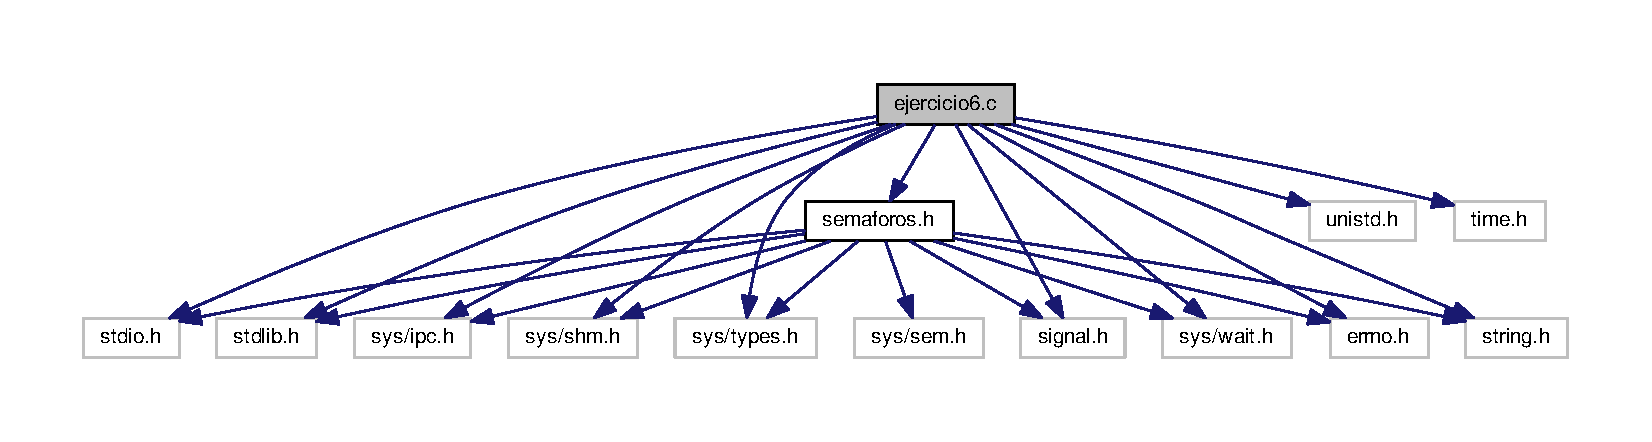
\includegraphics[width=350pt]{ejercicio6_8c__incl}
\end{center}
\end{figure}
\subsection*{\textquotesingle{}defines\textquotesingle{}}
\begin{DoxyCompactItemize}
\item 
\#define {\bfseries M\+A\+X\+B\+UF}~26\hypertarget{ejercicio6_8c_ad7871643c05865c80f5d8050aead2b57}{}\label{ejercicio6_8c_ad7871643c05865c80f5d8050aead2b57}

\item 
\#define {\bfseries P\+R\+O\+J\+ID}~1300\hypertarget{ejercicio6_8c_a489440928d1b279bb8bdc0bb2ccd414f}{}\label{ejercicio6_8c_a489440928d1b279bb8bdc0bb2ccd414f}

\end{DoxyCompactItemize}
\subsection*{Funciones}
\begin{DoxyCompactItemize}
\item 
int {\bfseries main} (int argc, char $\ast$argv\mbox{[}$\,$\mbox{]})\hypertarget{ejercicio6_8c_a0ddf1224851353fc92bfbff6f499fa97}{}\label{ejercicio6_8c_a0ddf1224851353fc92bfbff6f499fa97}

\end{DoxyCompactItemize}


\subsection{Descripción detallada}
Fuente del ejercicio 6. 

En este programa se simula el problema clásico del productor-\/consumidor, un proceso \char`\"{}produce\char`\"{} (escribe en una memoria compartida) y otro \char`\"{}consume\char`\"{} lo que se ha prducido (lee de la memoria compartida lo que ha escrito el productor)

\begin{DoxyAuthor}{Autor}
Juan Riera Gomez (\href{mailto:juan.riera@estudiante.uam.es}{\tt juan.\+riera@estudiante.\+uam.\+es}) y Carlos Ignacio Isasa Martín (\href{mailto:carlos.isasa@estudiante.uam.es}{\tt carlos.\+isasa@estudiante.\+uam.\+es}) 
\end{DoxyAuthor}
\begin{DoxyVersion}{Versión}
1.\+0 
\end{DoxyVersion}
\begin{DoxyDate}{Fecha}
07-\/abril-\/2017 
\end{DoxyDate}

\hypertarget{semaforos_8c}{}\section{Referencia del Archivo semaforos.\+c}
\label{semaforos_8c}\index{semaforos.\+c@{semaforos.\+c}}


Fuente del ejercicio 4.  


{\ttfamily \#include $<$stdio.\+h$>$}\\*
{\ttfamily \#include $<$stdlib.\+h$>$}\\*
{\ttfamily \#include $<$errno.\+h$>$}\\*
{\ttfamily \#include \char`\"{}semaforos.\+h\char`\"{}}\\*
Dependencia gráfica adjunta para semaforos.\+c\+:
\nopagebreak
\begin{figure}[H]
\begin{center}
\leavevmode
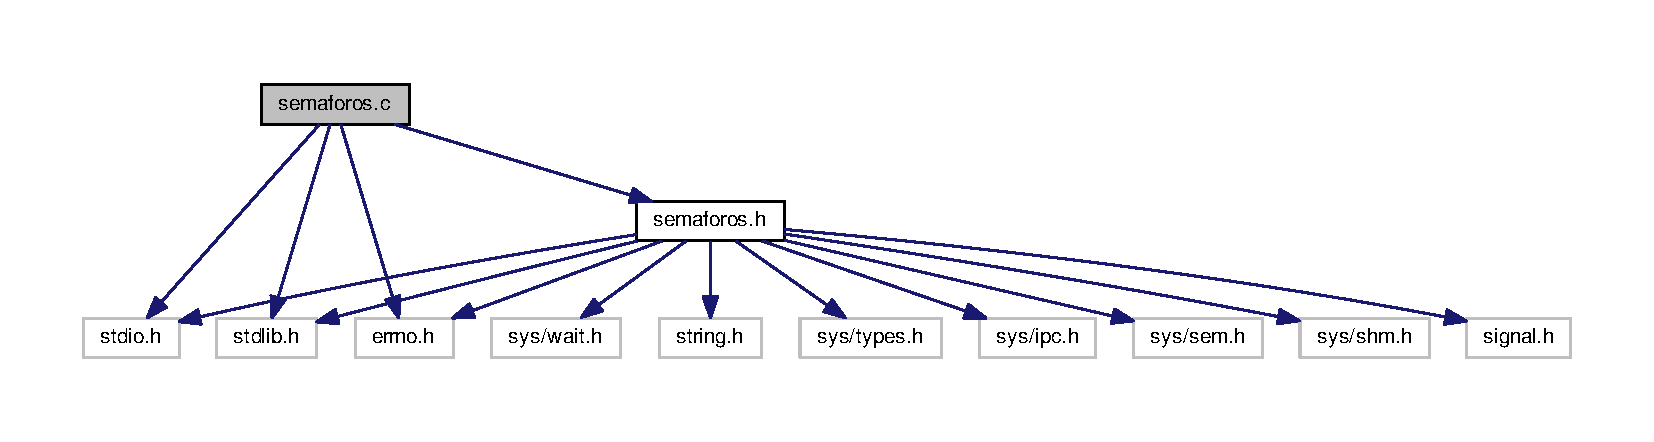
\includegraphics[width=350pt]{semaforos_8c__incl}
\end{center}
\end{figure}
\subsection*{Funciones}
\begin{DoxyCompactItemize}
\item 
int {\bfseries Inicializar\+\_\+\+Semaforo} (int semid, unsigned short $\ast$array)\hypertarget{semaforos_8c_a4af104b0ed37e6ae0289a1059bc6e990}{}\label{semaforos_8c_a4af104b0ed37e6ae0289a1059bc6e990}

\item 
int {\bfseries Borrar\+\_\+\+Semaforo} (int semid)\hypertarget{semaforos_8c_a731339337960a681efa435a10f12c312}{}\label{semaforos_8c_a731339337960a681efa435a10f12c312}

\item 
int {\bfseries Crear\+\_\+\+Semaforo} (key\+\_\+t key, int size, int $\ast$semid)\hypertarget{semaforos_8c_a16b16dd895b5f4cbe48f1ac8977e8b35}{}\label{semaforos_8c_a16b16dd895b5f4cbe48f1ac8977e8b35}

\item 
int {\bfseries Down\+\_\+\+Semaforo} (int id, int num\+\_\+sem, int undo)\hypertarget{semaforos_8c_a883244cd3b83c42cda23687da1b63369}{}\label{semaforos_8c_a883244cd3b83c42cda23687da1b63369}

\item 
int {\bfseries Down\+Multiple\+\_\+\+Semaforo} (int id, int size, int undo, int $\ast$active)\hypertarget{semaforos_8c_ab375ebfc38acbdced46e062a689d5fad}{}\label{semaforos_8c_ab375ebfc38acbdced46e062a689d5fad}

\item 
int {\bfseries Up\+\_\+\+Semaforo} (int id, int num\+\_\+sem, int undo)\hypertarget{semaforos_8c_a2d5e735aecee4f493898b3d4ebab1a10}{}\label{semaforos_8c_a2d5e735aecee4f493898b3d4ebab1a10}

\item 
int {\bfseries Up\+Multiple\+\_\+\+Semaforo} (int id, int size, int undo, int $\ast$active)\hypertarget{semaforos_8c_a943759695f018d64a94b8a2c49308092}{}\label{semaforos_8c_a943759695f018d64a94b8a2c49308092}

\end{DoxyCompactItemize}


\subsection{Descripción detallada}
Fuente del ejercicio 4. 

En este fuente se implementa la librería de semáforos propuesta en el enunciado.

\begin{DoxyAuthor}{Autor}
Juan Riera Gomez (\href{mailto:juan.riera@estudiante.uam.es}{\tt juan.\+riera@estudiante.\+uam.\+es}) y Carlos Ignacio Isasa Martín (\href{mailto:carlos.isasa@estudiante.uam.es}{\tt carlos.\+isasa@estudiante.\+uam.\+es}) 
\end{DoxyAuthor}
\begin{DoxyVersion}{Versión}
1.\+0 
\end{DoxyVersion}
\begin{DoxyDate}{Fecha}
06-\/abril-\/2017 
\end{DoxyDate}

\hypertarget{semaforos_8h}{}\section{Referencia del Archivo semaforos.\+h}
\label{semaforos_8h}\index{semaforos.\+h@{semaforos.\+h}}


Fuente del ejercicio 4.  


{\ttfamily \#include $<$stdio.\+h$>$}\\*
{\ttfamily \#include $<$stdlib.\+h$>$}\\*
{\ttfamily \#include $<$sys/shm.\+h$>$}\\*
{\ttfamily \#include $<$signal.\+h$>$}\\*
{\ttfamily \#include $<$sys/wait.\+h$>$}\\*
{\ttfamily \#include $<$errno.\+h$>$}\\*
{\ttfamily \#include $<$string.\+h$>$}\\*
{\ttfamily \#include $<$sys/types.\+h$>$}\\*
{\ttfamily \#include $<$sys/ipc.\+h$>$}\\*
{\ttfamily \#include $<$sys/sem.\+h$>$}\\*
Dependencia gráfica adjunta para semaforos.\+h\+:
\nopagebreak
\begin{figure}[H]
\begin{center}
\leavevmode
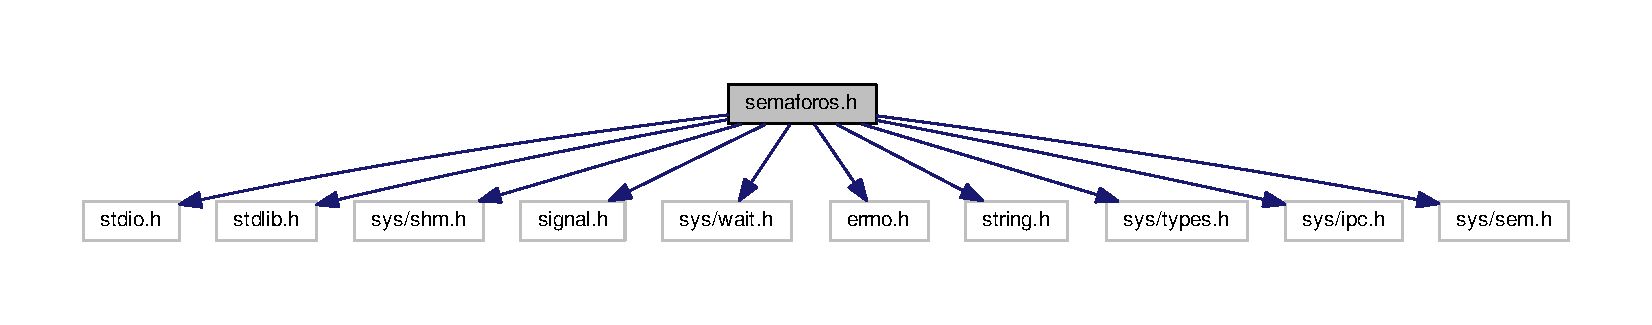
\includegraphics[width=350pt]{semaforos_8h__incl}
\end{center}
\end{figure}
Gráfico de los archivos que directa o indirectamente incluyen a este archivo\+:
\nopagebreak
\begin{figure}[H]
\begin{center}
\leavevmode
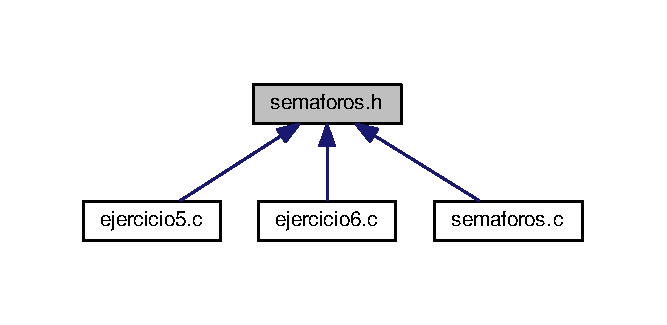
\includegraphics[width=320pt]{semaforos_8h__dep__incl}
\end{center}
\end{figure}
\subsection*{\textquotesingle{}defines\textquotesingle{}}
\begin{DoxyCompactItemize}
\item 
\#define {\bfseries OK}~0\hypertarget{semaforos_8h_aba51915c87d64af47fb1cc59348961c9}{}\label{semaforos_8h_aba51915c87d64af47fb1cc59348961c9}

\item 
\#define {\bfseries E\+R\+R\+OR}~-\/1\hypertarget{semaforos_8h_a8fe83ac76edc595f6b98cd4a4127aed5}{}\label{semaforos_8h_a8fe83ac76edc595f6b98cd4a4127aed5}

\end{DoxyCompactItemize}
\subsection*{Funciones}
\begin{DoxyCompactItemize}
\item 
int {\bfseries Inicializar\+\_\+\+Semaforo} (int semid, unsigned short $\ast$array)\hypertarget{semaforos_8h_a4af104b0ed37e6ae0289a1059bc6e990}{}\label{semaforos_8h_a4af104b0ed37e6ae0289a1059bc6e990}

\item 
int {\bfseries Borrar\+\_\+\+Semaforo} (int semid)\hypertarget{semaforos_8h_a731339337960a681efa435a10f12c312}{}\label{semaforos_8h_a731339337960a681efa435a10f12c312}

\item 
int {\bfseries Crear\+\_\+\+Semaforo} (key\+\_\+t key, int size, int $\ast$semid)\hypertarget{semaforos_8h_a16b16dd895b5f4cbe48f1ac8977e8b35}{}\label{semaforos_8h_a16b16dd895b5f4cbe48f1ac8977e8b35}

\item 
int {\bfseries Down\+\_\+\+Semaforo} (int id, int num\+\_\+sem, int undo)\hypertarget{semaforos_8h_a883244cd3b83c42cda23687da1b63369}{}\label{semaforos_8h_a883244cd3b83c42cda23687da1b63369}

\item 
int {\bfseries Down\+Multiple\+\_\+\+Semaforo} (int id, int size, int undo, int $\ast$active)\hypertarget{semaforos_8h_ab375ebfc38acbdced46e062a689d5fad}{}\label{semaforos_8h_ab375ebfc38acbdced46e062a689d5fad}

\item 
int {\bfseries Up\+\_\+\+Semaforo} (int id, int num\+\_\+sem, int undo)\hypertarget{semaforos_8h_a2d5e735aecee4f493898b3d4ebab1a10}{}\label{semaforos_8h_a2d5e735aecee4f493898b3d4ebab1a10}

\item 
int {\bfseries Up\+Multiple\+\_\+\+Semaforo} (int id, int size, int undo, int $\ast$active)\hypertarget{semaforos_8h_a943759695f018d64a94b8a2c49308092}{}\label{semaforos_8h_a943759695f018d64a94b8a2c49308092}

\end{DoxyCompactItemize}


\subsection{Descripción detallada}
Fuente del ejercicio 4. 

En este fuente tenemos el header asociado a la librería de semáforos \textquotesingle{}\hyperlink{semaforos_8c}{semaforos.\+c}\textquotesingle{}.

\begin{DoxyAuthor}{Autor}
Juan Riera Gomez (\href{mailto:juan.riera@estudiante.uam.es}{\tt juan.\+riera@estudiante.\+uam.\+es}) y Carlos Ignacio Isasa Martín (\href{mailto:carlos.isasa@estudiante.uam.es}{\tt carlos.\+isasa@estudiante.\+uam.\+es}) 
\end{DoxyAuthor}
\begin{DoxyVersion}{Versión}
1.\+0 
\end{DoxyVersion}
\begin{DoxyDate}{Fecha}
06-\/abril-\/2017 
\end{DoxyDate}

%--- End generated contents ---

% Index
\backmatter
\newpage
\phantomsection
\clearemptydoublepage
\addcontentsline{toc}{chapter}{Índice}
\printindex

\end{document}
